

\author[Sebastian Hahn]{Nix}


\beamertemplatenavigationsymbolsempty{}

\logo{
\includegraphics[height=1cm]{Bilder/logo}}


\newcommand{\qenc}{q_{\boldsymbol\phi}(\mathbf{z}|\mathbf{x}_i)}
\newcommand{\qencd}{q_{\phi}(z|x_i}
\newcommand{\penc}{p_{\boldsymbol\theta}(\mathbf{z}|\mathbf{x}_i)}
\newcommand{\pdec}{p_{\boldsymbol\theta}(\mathbf{x}_i|\mathbf{z})}
\newcommand{\tx}{\widetilde{x}}
\newcommand{\tz}{\widetilde{z}}
\newcommand{\tZ}{\widetilde{Z}}
\newcommand{\tX}{\widetilde{X}}
\newcommand{\tmu}{\widetilde{\mu}}
\newcommand{\tsig}{\widetilde{\sigma}}
\newcommand{\bP}{\mathbb{P}}
\newcommand{\bbf}{\bold{f}}
\newcommand{\bmu}{\bm{\mu}}
\newcommand{\bsig}{\bm{\sigma}}
\newcommand{\z}{\mathbf{z}}
\newcommand{\x}{\mathbf{x}_i}


\section{Sektion-Überschrift}

\begin{frame}
	\frametitle{VAE - Verlustfunktion}
	\begin{align*}
	\log\big(p_{\boldsymbol\theta}(\x)\big) - \underbrace{D_{KL}\big[\qenc || \penc\big]}_{\ge 0}
	\end{align*}
	\begin{align*}
	=\underbrace{ \E_{\z\sim q_{\boldsymbol\phi}}\big[\log\big(\pdec\big)\big] - D_{KL}\big[\qenc||p_{\boldsymbol\theta}(\z)\big]}_{=:\ \mathrm{ELBO}\ =\ -\mathcal{L}(\boldsymbol\theta,\boldsymbol\phi,\mathbf{x}_i)}
	\end{align*}
\end{frame}

\begin{frame}
	\frametitle{VAE}
	\begin{figure}
	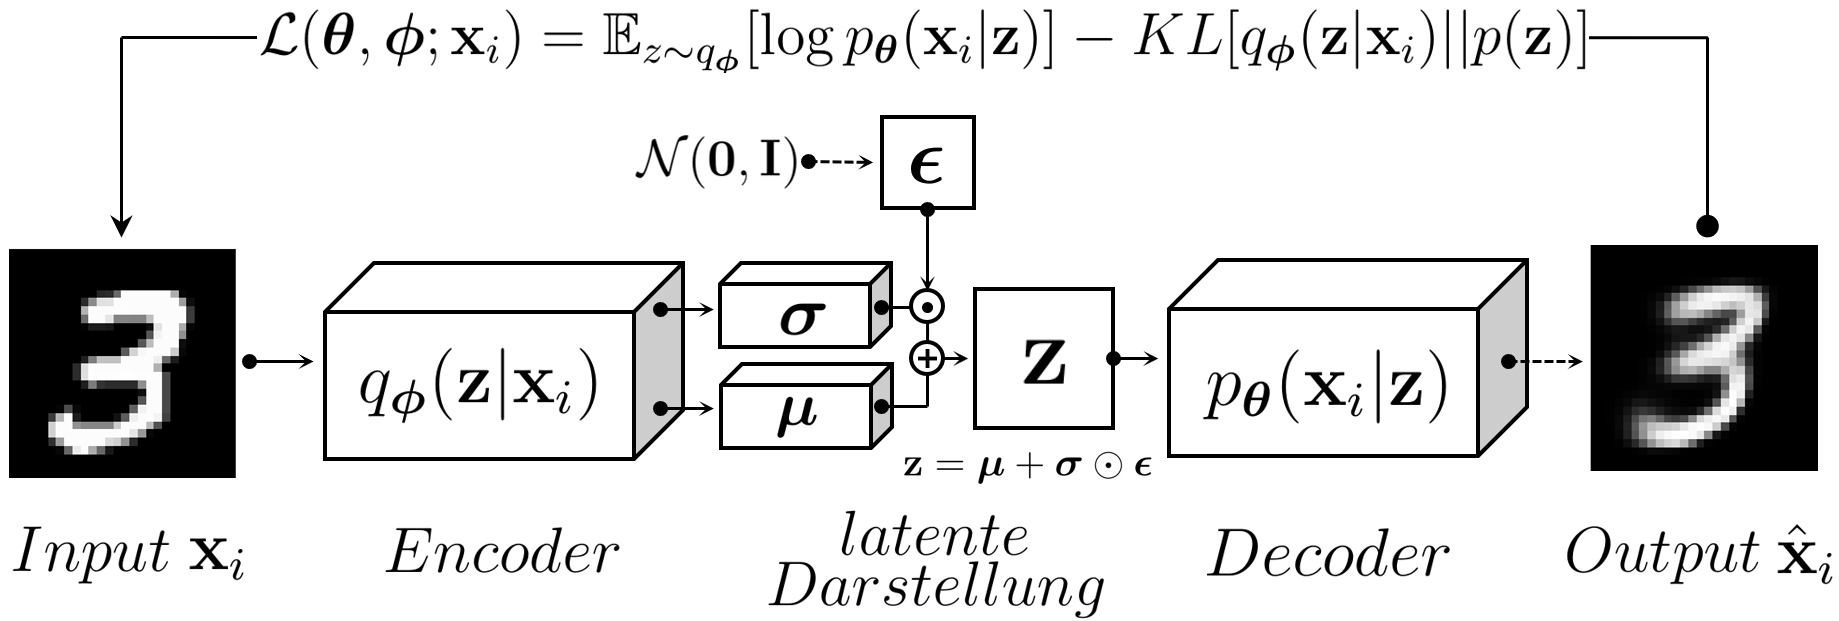
\includegraphics[scale=0.27]{Bilder/VAE-Modell.PNG}
	\end{figure}
\end{frame}

\begin{frame}
	\frametitle{Beispiel eines latenten Raumes}
	
	\begin{figure}[h!]
		\centering
		\begin{minipage}{.6\textwidth}
			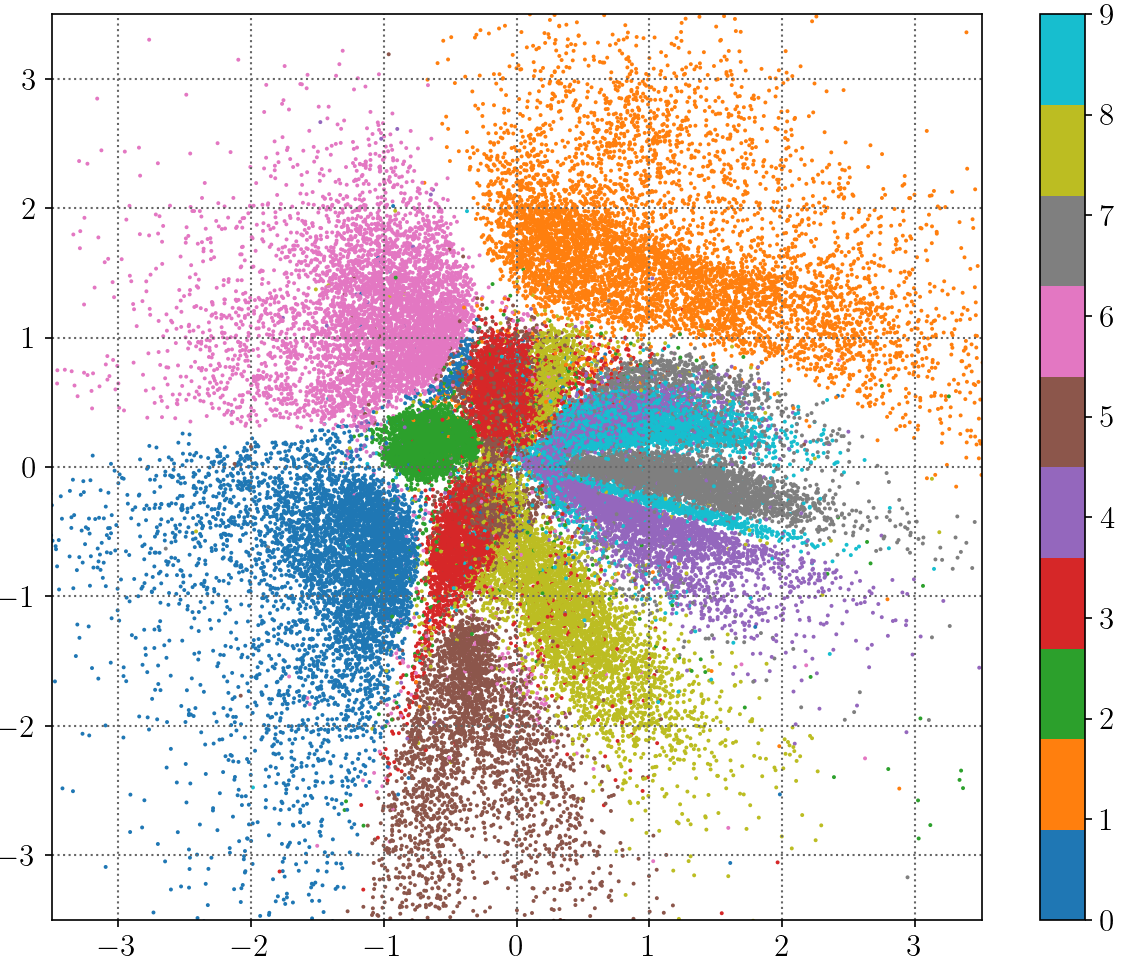
\includegraphics[scale=0.28]{Bilder/latent_space_2D.png}
		\end{minipage}%
		\begin{minipage}{.5\textwidth}
			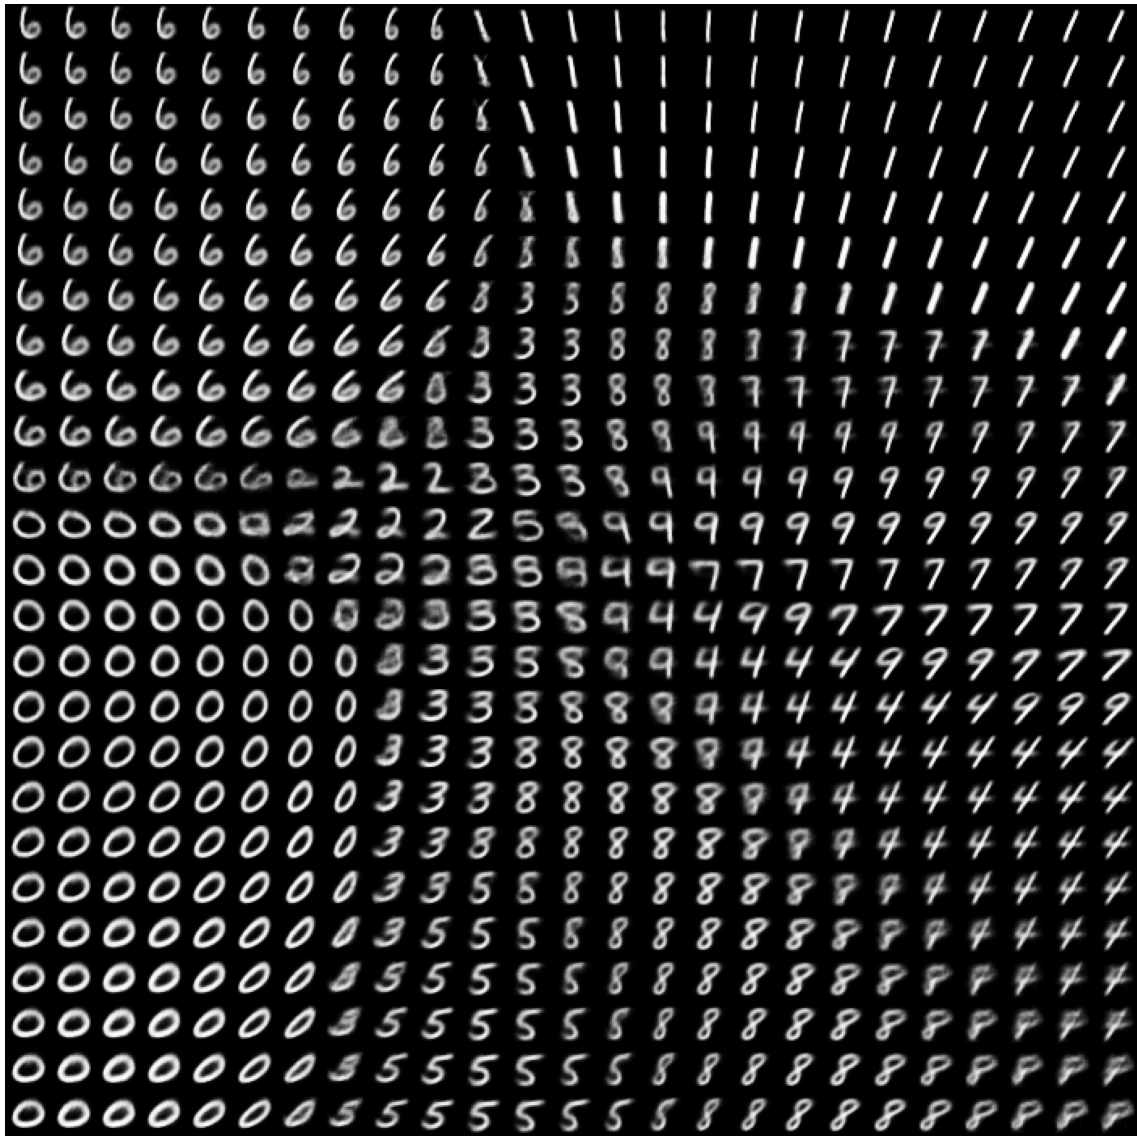
\includegraphics[scale=0.23]{Bilder/latent_space_2D_reconstructions.png}
		\end{minipage}
	\end{figure}
\end{frame}
